% !TeX root = ../main.tex

\chapter{Classification of Algorithms}
	\begin{statement}
		Algorithms are the most important and durable part of computer science. However in order to use them effectively we need a way of evaluating efficiency without implementing them in software.
		
	\end{statement}


Imagine you had an problem that involved taking a list of items and spat them out after doing some arbitrary processing. You have a selection of algorithms that would be appropriate for this task, but how would you evaluate its performance? The simplest way would be implement each to run it over every possible combination of and measure how long it took. There are two issues with this approach, the first is that the majority of resources used in the implementation of the algorithms are wasted once one is selected. The second issue is that even for one algorithm, we have an infinite number of possible inputs. Lets say our list contains one item, there are an infinite number of values just between $0$ and $1$. Even if we limit ourselves to only using the numbers $1 ... n$ where $n$ is the number of inputs required we quickly run into the other issue that the number of possible combinations for this set is $n!$. For just 10 items there are $3,628,800$ combinations that we will have to try. Clearly this is unworkable when in most applications we are talking about data sets on the order of thousands. Clearly we need a method of being able to study algorithms without actually implementing them and testing them.

\section{Best, Worst and Average Case Complexity}
	\index{Complexity} Complexity is a measure of how a problem grows as the size increases \glossary{Complexity}. If we take a problem and run it over all possible arrangements of $n$ keys we can plot a graph (see fig. \ref{fig:bigOgraph}) where the $x$-axis represents the size of the input problem and the $y$-axis denotes the number of steps taken by the algorithm in this instance. We can then define three interesting functions over the plot of these points	
	\begin{itemize}
		\item The \textit{worst-case complexity} \index{Complexity!Worst Case} of the algorithm is the function defined by the maximum number of steps taken in any particular instance of size $n$. This represents the urver passing through the highest point in each column.
		\item The \textit{best-case complexity} \index{Complexity!Best Case} is the function defined by the minimum number of steps take in any instance of size $n$. This represents the curve passing through the lowest point of each column.
		
		\item The \textit{average-case complexity} \index{Complexity!Average Case}  of the algorithm, which is the function defined by the average number of steps over all instances of size $n$.
	\end{itemize}
	\begin{figure}[t]
		\centering
		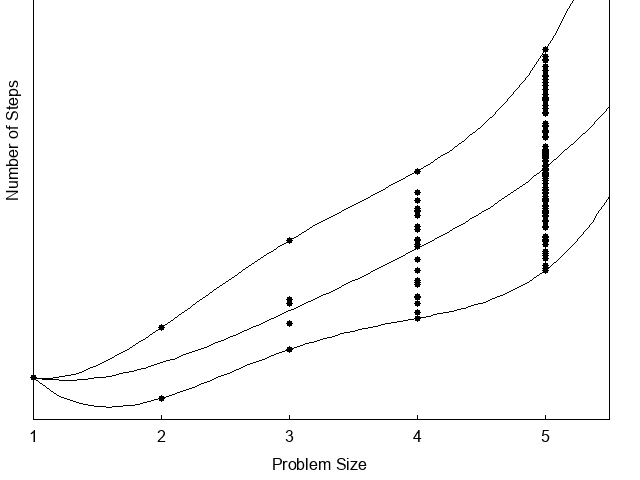
\includegraphics[width=0.75\textwidth]{./assets/imgs/bigOcomplexity.png}
		\caption{\label{fig:bigOgraph} Best, worst and average-case complexity}
	\end{figure}
	
	The worst-case complexity turns out to be the most useful of these measures in practice. At first glance this might seem counter-intuitive Perhaps the best analogy is think about what happens if you bring £$n$ into a casino to gamble. The best case is that you walk out owning the place, it is possible but is so unlikely that you should not even think about it. The worst case, that you lose all $n$ dollars is easy to calculate and distressingly likley to happen. The average case, that the typical bettor loses \SI{87.32}{\percent} of the money that they bring into the casino, is difficult to establish and its meaning is subject to debate. What exactly does \textit{average} mean? Stupid people loose more that smart people, so are you smarter or stupider than the average person, and by how much? Card counters at blackjack do better on average than customers that accept three or more free drinks. It is far easier to avoid all of these complexities and obtain a very useful result just by considering the worst case.
	
	The last important thing to realise is that each of these time complexities define a numerical function, representing time versus problem size. These functions are as well defined as any other numerical function, be it $y = x^2 - 2x + 1$ or the price of a particular stock as a function of time. However time complexities are such complex functions that we must simplify them to work with.  For this we need \enquote{Big Oh} notation. 
\section{Big Oh Notation}
\index{Big Oh Notation}
  The issue with using numerical functions when doing complexity analysis tends to be two fold:
  \begin{itemize}
  	\item \textit{They have two many bumps} - An algorithm such as binary search typically runs a bit faster for arrays of size $n = 2^k - 1$ (where $k$ is an integer), because the array partitions works out nicely. Whilst this detail is not particularly significant, it does mean that the \textit{exact} complexity function is likely to be very complicated, with little up and down bumps. 
  	\item \textit{Requires too much detail to specify precisely} - Counting the exact number of RAM instructions executed in the worst case requires that the algorithm be specified to the detail of a complete computer program. This means that individual foibles of the programming language start to creep in, e.g. the peformance of a \texttt{case} statement in C vs a nested if in Python would start to play a role.  
  \end{itemize}

	\subsection{Formal Definition}
		\begin{figure}[t]
			\centering
			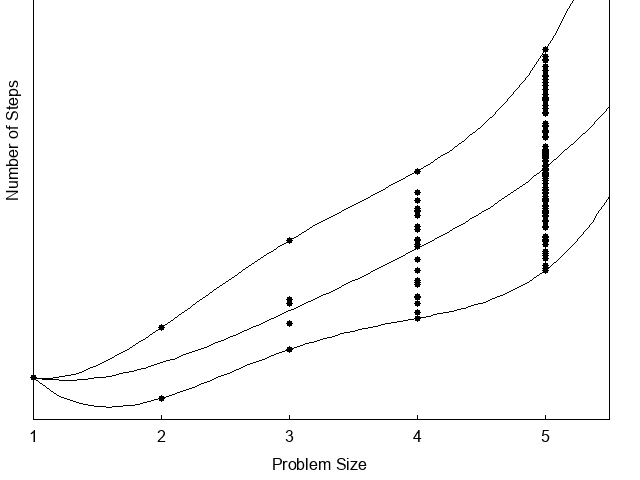
\includegraphics[width=0.75\textwidth]{./assets/imgs/bigOcomplexity.png}
			\caption{\label{fig:bigOdefiniton} Illustrating the Big Oh notations}
		\end{figure}
		The formal definition of Big Oh states that	$f(n) = \mathcal{O}(g(n))$ means $c \cdot g(n)$ is an \textit{upper bound} on $f(n)$. Thus there exists some constant $c$ such that $f(n)$ is always $\le c \cdot g(n)$, for a large enough $n$ (i.e., $n \ge n_0$ for some constant $n_0$). \footnote{We should also add for completeness there is also a function $\Omega(g(n))$ which provides a lower bound, and $\Theta(g(n))$ that exists bounded between $\Omega(g(n))$ and Big Oh.}
		
		But what does that actually mean? First it assumes a constant $n_0$ beyond which they are always satisfied. This means we are not concerned about small values of $n$. This seems reasonable on two fronts: first, most programs take about the same time for $n\le10$ so we are not to concerned with performance; second, there more significant fluctuations that exist for low $n$. We are more concerned how our algorithm behaves at $n=\num{10000}$ and $n=\num{100000}$. Second it is not concerned with any multiplicative constants. The function $f(n) = 2n$ and $g(n) = n$ are identical in big Oh analysis for different values of $c$. Figure \ref{fig:bigOdefiniton} shows how we can draw an upper and lower bound on some function $f(n)$. 
		
		\begin{figure}[t]
			\centering
			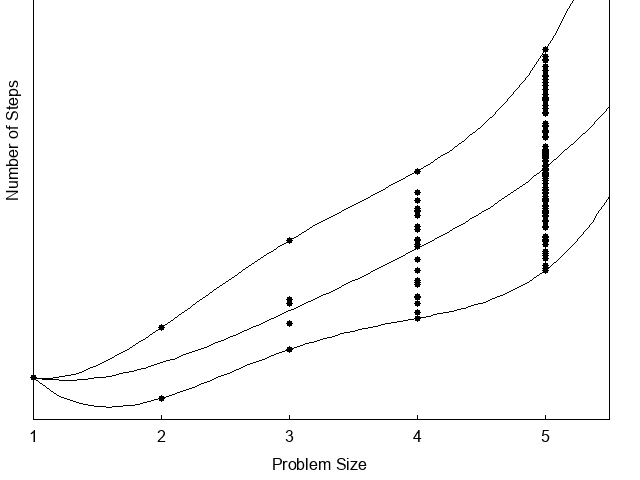
\includegraphics[width=0.75\textwidth]{./assets/imgs/bigOcomplexity.png}
			\caption{\label{fig:bigOExampleGraph} Fitting a function to f(n) for a variety of constants}
		\end{figure}
	
		As an example lets take the function $3n^2 - 100n + 6$, which we've plotted in \ref{fig:bigOExampleGraph}, and try and work out what its big Oh notation is.
		
		\begin{equation}
			3n^2 - 100 + 6 = \bigo{n^2}, \text{for}\: c = 3 \because 3n^2 > 3n^2 - 100n + 6 
		\end{equation}
		\begin{equation}	
			3n^2 - 100 + 6 = \bigo{n^3}, \text{for}\: c = 1 \because n^3 > 3n^2 - 100n + 6\: \text{when}\: n > 3 
		\end{equation}
		\begin{equation}	
			3n^2 - 100 + 6 \ne \bigo{n}, \forall c \because c \cdot n < 3n^2, \text{when}\: n>c
		\end{equation}
		
		The slightly confusing part is when you see the expression $n^2 = \bigo{n^3}$, but if you go back to the definitions and remember that Big Oh is defined in terms of an \textit{upper bound}. This means that we can read the \enquote{=} here as meaning \textit{one of the functions that are}. Clearly $n^2$ is one of the functions that are \bigO{n^3}.
	 
	\subsection{Grow Rates and Dominance Relations}
		With the Big Oh notation, we discard the multiplicative constants, thus the functions $f(n) = 0.001n^2$ and $g(n) = 1000n^2$ are treated identically, even though $g(n)$ is a million times larger than $f(n)$ for all values of $n$. The reason why we are content with the fairly coarse analysis provided in Table \ref{tab:BigOComparison}, which shows the growth rate of several common time analysis functions. In particular it shows how long algorithms that use $f(n)$ operations take to run on a computer that executes one instruction in \SI{1}{\ns} (e.g. \SI{1}{\giga\hertz}). We can draw the following conclusions:
		
		\begin{itemize}
			\item All such algorithms take roughly the same time for $n = 10$
			\item Any algorithm with $n!$ running time becomes useless for $n\ge 20$.
			\item Algorithm whose running time is $2^n$ have a greater operating range, but become impractical for $n>40$.
			\item Quadratic-time algorithms remain usable up to about $n = \num{10000}$, but quickly deteriorate with larger inputs.
			\item Linear-time and $n \lg n$ algorithms remain practical on inputs of one billion item.
			\item A \bigO{\lg n} algorithm hardly breaks a sweat for any imaginable value of $n$.
		\end{itemize}
	
	The bottom line is that despite ignoring constant factors, we get an excellent idea of whether a given algorithm is appropriate for a problem of a given size. 
	
		\subsubsection{Dominance Relations}
			We can group Big notation into a set of classes, such that all the functions in a particular class are equivalent in respect to Big Oh. We say that a faster growing function \textit{dominates} a slower-growing one. Below we shall list the most common function classes in order of increasing dominance.
			%TODO: Expand this Section
			\begin{description}
				\item[Constant functions, $f(n) = 1$] Such functions might measure the cost of adding two numbers, printing out the lyrics to a song, or inserting into a sorted array. There is no dependence on the size of $n$.
				\item[Logarithmic functions, $f(n) = \log n$] This turns up in algorithms such as binary search. They grow quite slowly as $n$ gets big but faster than the constant function.
				\item[Linear functions, $f(n) = n$] Such functions measure the cost of looking at each item once (or twice, or ten times) in an $n$-element array, say to compute the average value.
				\item[Superlinear functions, $f(n) = n \log n$] This class of functions arises in algorithms such as Quicksort and Mergesort.
				\item[Quadratic functions, $f(n) = n^2$] These measure the cost of looking at most or all \textit{pairs} of items in an $n$-element universe. This arises in algorithms such as insertion and selection sort.
				\item[Cubic functions, $f(n) = n^3$] These functions enumerate over all triples of items in an $n$-element universe. 
				\item[Exponential functions, $f(n) = c^n \forall c > 1$] Functions like $2^n$ arise when enumerating all subsets of n items.
				\item[Factiorial functions, $f(n) = n!$] Functions like this arise when generating all permutations or orderings of $n$ items.
			\end{description}
			\begin{figure}[t]
				\centering
				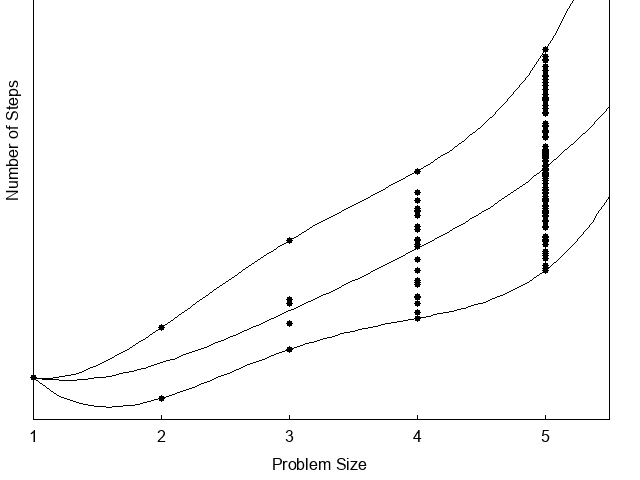
\includegraphics[width=0.8\textwidth]{./assets/imgs/bigOcomplexity.png}
				\caption{\label{fig:bigODominanceRelationships} The growth rates of various common functions}
			\end{figure}			
			Figure \ref{fig:bigODominanceRelationships} shows these graphically. We'll discuss the importance of dominance relationships in the next section. However the important thing to understand is:
			\begin{equation}
				n! \gg c^n \gg n^3 \gg n^2 \gg n \log n \gg n \gg \log n \gg 1
			\end{equation}
		As a shorthand we often refer to problems that have polynomial or less solutions are known as traceable problems and ones with greater than polynomial solutions are called in-traceable.
\begin{table}[t]
	\centering
	\begin{tabular}{>{\scriptsize}L{0.15\linewidth} | >{\scriptsize}L{0.10\linewidth} >{\scriptsize}L{0.10\linewidth} >{\scriptsize}L{0.10\linewidth} >{\scriptsize}L{0.10\linewidth} >{\scriptsize}L{0.10\linewidth} >{\scriptsize}L{0.10\linewidth}}
		\renewcommand{\arraystretch}{0.1}
		$n$				& $\lg n$	& $n$		& $n \lg n$	& $n^2$		& $2^n$		& $n!$		\\
		\hline \hline
		$\num{10}$ 			& \SI{0.003}{\us}	& \SI{0.01}{\us}	& \SI{0.033}{\us}	& \SI{0.1}{\us}		& \SI{1}{\us}		& \SI{3.63}{\ms} 		\\
		$\num{20}$			& \SI{0.004}{\us}	& \SI{0.02}{\us}	& \SI{0.086}{\us}	& \SI{0.4}{\us}		& \SI{1}{\ms}		& \SI{77.1}{\year}		\\
		$\num{30}$			& \SI{0.005}{\us}	& \SI{0.03}{\us}	& \SI{0.147}{\us}	& \SI{0.9}{\us}		& \SI{1}{\s}		& \SI{8.4e15}{\year}	\\
		$\num{40}$			& \SI{0.005}{\us}	& \SI{0.04}{\us}	& \SI{0.213}{\us}	& \SI{1.6}{\us}		& \SI{18.3}{\min}	&						\\
		$\num{50}$			& \SI{0.006}{\us}	& \SI{0.05}{\us}	& \SI{0.282}{\us}	& \SI{2.5}{\us}		& \SI{13}{\day}		&						\\
		\hline
		$\num{100}$			& \SI{0.007}{\us}	& \SI{0.1}{\us}		& \SI{0.644}{\us}	& \SI{10}{\us}		& \SI{4e13}{\year}	&						\\
		$\num{1000}$		& \SI{0.010}{\us}	& \SI{1}{\us}		& \SI{9.966}{\us}	& \SI{1}{\ms}		&					&						\\
		$\num{10000}$		& \SI{0.013}{\us}	& \SI{10}{\us}		& \SI{130}{\us}		& \SI{100}{\ms}		&					&						\\
		$\num{100000}$		& \SI{0.017}{\us}	& \SI{0.10}{\ms}	& \SI{1.67}{\ms}	& \SI{10}{\s}		&					&						\\
		$\num{1000000}$		& \SI{0.020}{\us}	& \SI{1}{\ms}		& \SI{19.93}{\ms}	& \SI{16.7}{\minute}&					&						\\
		$\num{10000000}$	& \SI{0.023}{\us}	& \SI{0.01}{\s}		& \SI{0.23}{\s}		& \SI{1.16}{\day}	&					&						\\
		$\num{100000000}$	& \SI{0.027}{\us}	& \SI{0.1}{\s}		& \SI{2.66}{\s}		& \SI{115.7}{\day}	&					&						\\
		$\num{1000000000}$	& \SI{0.030}{\us}	& \SI{1}{\s}		& \SI{29.90}{\s}	& \SI{31.7}{\year}	&					&						\\
	\end{tabular}
	\caption{\label{tab:BigOComparison} A Comparison of the worst case performances of different implementations of a Dictionary for different operations.}
\end{table}
	\subsection{Working with the Big Oh}
		When reasoning what Big Oh class different 	
		\subsubsection{Adding Functions}
			The sum of two functions is governed by the dominant one, i.e
			\begin{equation}\label{equ:bigOaddingdominance}
				\bigo{f(n)} + \bigo{g(n)} \rightarrow \bigo{\max(f(n),g(n))}
			\end{equation}
		
		\subsubsection{Multiplying Functions}
			There are two types of multiplication that we need to worry about with Big Oh, the first is with a constant factor, the second is with a second function. With a constant the answer is simple, you just ignore it as in Equation \ref{equ:bigOmultiplicationconstant}. Obviously this doesn't hold for $c \ge 0$ as multiplying even \bigO{n!!} is quickly wiped out if you multiply it by zero, but for most cases we will come across this will not be the case.
			
			\begin{equation}\label{equ:bigOmultiplicationconstant}
				\bigo{c \cdot f(n)} \rightarrow \bigo{f(n)}
			\end{equation}
			
			However for when you are multiplying a function by another function both results are important. This leads to the result in Equation \ref{equ:bigOmultiplicationfunction}. 
			
			\begin{equation}\label{equ:bigOmultiplicationfunction}
				\bigo{f(n)} \cdot \bigo{g(n)} \rightarrow \bigo{f(n) \cdot g(n)}
			\end{equation}
			e.g.
			\begin{equation}\label{equ:bigOmultiplicationfunctionexample}
			\bigo{n^2} \cdot \bigo{\log n} \rightarrow \bigo{n^2 \log n}
			\end{equation}
			
		

			
	\subsection{Example Derivation}
		In this section we are going to reason our way through some common algorithms and see if we can derive the big Oh notation for a given algorithm.
		\subsubsection{String Pattern Matching}
			Pattern matching is the most fundamental algorithm that we perform on text strings. This algorithm implements the find command available in any web browser or text editor.
			
			\textit{Problem:} Substring Pattern Matching
			\textit{Input:} A text string $t$ and a pattern string $p$.
			\textit{Output:} Does $t$ contain the pattern $p$, and if so where?
			
			\begin{figure}[h]
\begin{minted}{c}
int findmatch(char *p, char *t) {
	int i, j;		/* counters */
	int m, n;		/* string lengths */
	
	m = strlen(p);
	n = strlen(t);
	
	for (i=0; i <= (n - m); i++) {
		j = 0;
		while((j < m) && (t[i+j] == p[j])) {
			j = j+1;
		}
		if (j == m) {
			return(i);			
		}
	}
	
	return(-1);
}
\end{minted}
				\caption{\label{code:findmatch} Algorithm for finding a matching string.}
				\index{Strings!Substring}
			\end{figure}
				
			What is the worst-case running time of these two nested loops? The inner \textit{while} looop goes around at most $m$ times, and potentially far less when the pattern match fails. The outer loop goes around at most $n-m$ times, since no complete match can be found once there are not enough characters left. With nested loops we multiply the complexity \footnote{This is because every time we run the outer the loop we run the complete inner loop} so we get a worst case complexity given in equation \ref{equ:findmatch1}, the $+2$ refers to the two extra statements that are within the outer \textit{for} loop.
			
			\begin{equation}\label{equ:findmatch1}
				\bigo{(n-m)(m + 2)}
			\end{equation}
			
			We also need to consider the time taken to find the length of each of the strings. Lets just assume that we explicitly count the number of characters until we hit the end of the string, this suggests that it would take linear time. So the total running time would be given in equation \ref{equ:findmatch2}
			\begin{equation}\label{equ:findmatch2}
			\bigo{n+m+(n-m)(m + 2)}
			\end{equation}
			
			Simplifying the constant term,
			\begin{equation}\label{equ:findmatch3}
			\bigo{n+m+(n-m)m}
			\end{equation}
			
			Multiplying it out,
			\begin{equation}\label{equ:findmatch4}
			\bigo{n+m+nm-m^2}
			\end{equation}
			
			We know that $n \ge m$ because a sub string that longer than the original text would be impossible. So,
			\begin{equation}\label{equ:findmatch5}
			n + m \le 2n \rightarrow \bigo{n}
			\end{equation}
			Substituting \ref{equ:findmatch5} in leaves:
			\begin{equation}\label{equ:findmatch6}
			\bigo{n+nm-m^2}
			\end{equation}
			We also note that $n \le nm$, since $m \ge 1$ for any interesting problem thus:
			\begin{equation}\label{equ:findmatch7}
			n + nm \rightarrow \bigo{nm}
			\end{equation}
			This allows us to drop the additive $n$ and leave us with Equation \ref{equ:findmatch8}
			\begin{equation}\label{equ:findmatch8}
			\bigo{nm-m^2}
			\end{equation}
			Finally we observe that the $-m^2$ term is negative so only serves to lower the value within. Because Big Oh is an upper bound, we can drop any negative without invaliding the output. We also know that because $n \ge m$, $ mn \ge m^2$ so it isn't big enough to cancel out any term that is left. This leaves a worst case complexity of \bigO{nm}
			
		\subsubsection{Matrix Multiplication}
			Matrix multiplication is a fundamental operation in linear algebra. 
			\textit{Problem:} Matrix Multiplication
			\textit{Input: } Two matrices, $A$ (dimensions $x \times y$) and $B$ (dimensions $y \times z$)
			\textit{Output: } A $x \times z$ matrix $C$ where $C[i][j]$ is the dot product of the $i$th row of $A$ and the $j$th column of $B$.
			
			\begin{figure}[h]
\begin{minted}{c}
for (i = 1; i <= x; i++) {
	for (j = 1; j <= z; j++) {
		C[i][j] = 0;
		for (k = 1; k <= y; k++) {
			C[i][j] += A[i][k] * B[k][j];		
		}
	}
}
\end{minted}
				\caption{\label{code:matrixmult} Multiplying two matrices, A and B to get C.}
			\end{figure}
		
			The number of multiplication operations is given by $M(x, y, z)$ which is the result of a nested summation shown in \ref{equ:matrixmult1}
			
			\begin{equation}\label{equ:matrixmult1}
				M(x,y,z) = \sum_{i=1}^{x} \sum_{j=1}^{y} \sum_{k=1}^{z} 1 	
 			\end{equation}
 			We evaluate from the right inward. The sum of $z$ ones is $z$ so:
 			\begin{equation}\label{equ:matrixmult2}
	 			M(x,y,z) = \sum_{i=1}^{x} \sum_{j=1}^{y} z
	 		\end{equation}
	 		\begin{equation}\label{equ:matrixmult3}
	 			M(x,y,z) = \sum_{i=1}^{x}yz
	 		\end{equation}
		 	\begin{equation}\label{equ:matrixmult4}
	 			M(x,y,z) = xyz
 			\end{equation}
	 		
	 		Thus the running of a matrix multiplication \index{Matrix Multiplication} is \bigO{xyz}, for the case that $x = y = z$ we get \bigO{n^3} i.e. a cubic algorithm.
		\subsubsection{Binary Search and Logarithms}
			Binary Search \index{Binary Search} is a good example of an \bigO{\log n} algorithm. It is covered in more detail in section \ref{section:BinarySearch} but for now imagine you have a telephone book. You want to locate person, $p$ in a telephone book containing $n$ names. In a binary search you start by comparing it to the middle or \nicefrac{n}{2} name, say \textit{Monroe, Marilyn}. You then discard half the book depending if the name came before or after middle. You repeat this process until you get to having only one name left. The important question for our analysis is how many steps will it take to get down to this one name? 
			Lets start by turning the problem on its head. After $h$ comparisons how many different values could you have compared? For $h = 1$ the answer is trivial - 1. For $h = 2$, we have the first element that we compared and the two either that we jump to next. Fig \ref{fig:simpleBinaryTree} demonstrates how the number of items grows for $h$. We can work out that after $h$ jumps we can cover $2^h - 1$ items. Equation \ref{equ:binSearch1} shows how this is derived to get a complexity of \bigO{\lg n}
			\begin{gather}
				n = 2^h - 1 \label{equ:binSearch1} \\
				\lg n = \lg(2^h) - \lg 1 \label{equ:binSearch2} \\
				\lg n = h \label{equ:binSearch3}
			\end{gather}
			
			\begin{figure}[t]
				\centering
				\begin{tikzpicture}
					\draw[fill=black] (0,0) circle (0.05)  node[above] {\small Monroe, Marlyin};
					\draw[fill=black] (-3,-1) circle (0.05)  node[above] {\small Dean, James};
					\draw[fill=black] (3,-1) circle (0.05)  node[above] {\small Presly, Elvis};
					\draw[fill=black] (-4.5,-2) circle (0.05)  node[above] {\small Collins, Phil};
					\draw[fill=black] (-1.5,-2) circle (0.05)  node[above] {\small Hendrix, Jimmi};
					\draw[fill=black] (1.5,-2) circle (0.05)  node[above] {\small Parton, Dolly};
					\draw[fill=black] (4.5,-2) circle (0.05)  node[above] {\small Springsteen, Bruce};
					
					\draw[->] (-7,1)  node[above]  {$h$} -- +(0,-5);
					\draw (-7,0) -- +(-.2,0) node[left] {$1$};
					\draw (-7,-1) -- +(-.2,0) node[left] {$2$};
					\draw (-7,-2) -- +(-.2,0) node[left] {$3$};
					\draw (-7,-3) -- +(-.2,0) node[left] {$\dots$};
					\draw(0,0) -- (-1.75,-0.4);
					\draw(0,0) -- (1.75,-0.4);
					\draw(-3,-1) -- (-3.8,-1.4);
					\draw(3,-1) -- (3.8,-1.4);
					\draw(-3,-1) -- (-2.2,-1.4);
					\draw(3,-1) -- (2.2,-1.4);
				\end{tikzpicture}
				\caption{\label{fig:simpleBinaryTree} the results of a possible Binary Search after $h$ comparisons. }
			\end{figure}
	\section{Greedy Algorithms}
	
	\section{P vs NP Problems}
		One of the most profound open problems in computer science asks \enquote{Is $P = NP$?}. In simple language it is asking whether \textit{verification} is easier than initial \textit{discovery}. A good analogy is lets say during the course of an exam you happen to notice the answer of the student next to you. Are you now better off? You wouldn't turn it in without checking, since you could answer the question correctly if you took enough time to find it from scratch. The question is whether you can really verify the answer faster than you could find it from scratch. 
		
		In particular we are referring to two classes of problems: $P$ and $NP$. The class $P$ is an exclusive club that can only be joined whence a problem has demonstrated that there is a polynomial-time algorithm to solve it. A less-exclusive club welcomes all problems who can be \textit{verified} in polynomial time. This obviously includes all members P. We call this club $NP$ standing for \textit{non-deterministic polynomial time}. The question is whether problems in $NP$ that cannot be in $P$. Most people who actually study this field believe that $P \ne NP$ but haven't found a proof yet.
	
	\section{The Halting Problem}
		So far all the problems that we have covered
	\section{Turing Machines}
	
	\section{State Transition Diagrams}
	
	\section{Exercises}
		
		\subsection{Exam Style Questions}
			\begin{enumerate}
				\item What value is returned by the following function? Express your answer as a function of $n$. Give the worst-case running time using the Big Oh notation
			\end{enumerate}